\section{An experimental board for learning sequences of actions based on visual rewards}
\label{sec:serial_experimental_board}

One aspect of the extensive work described in this report was to give to encourage the robot to learn particular sequence of gazes/actions.

This would be achieved by using an experimental board which has been designed and developed by the IMCLeVeR consortium for this particular purpose, i.e. to be able to pre-program sequences of actions that lead to rewards. The board, which is shown in Figure~\ref{fig:experimental_board}, consists of two main types of modules:

\begin{figure}[htb]
\begin{center}
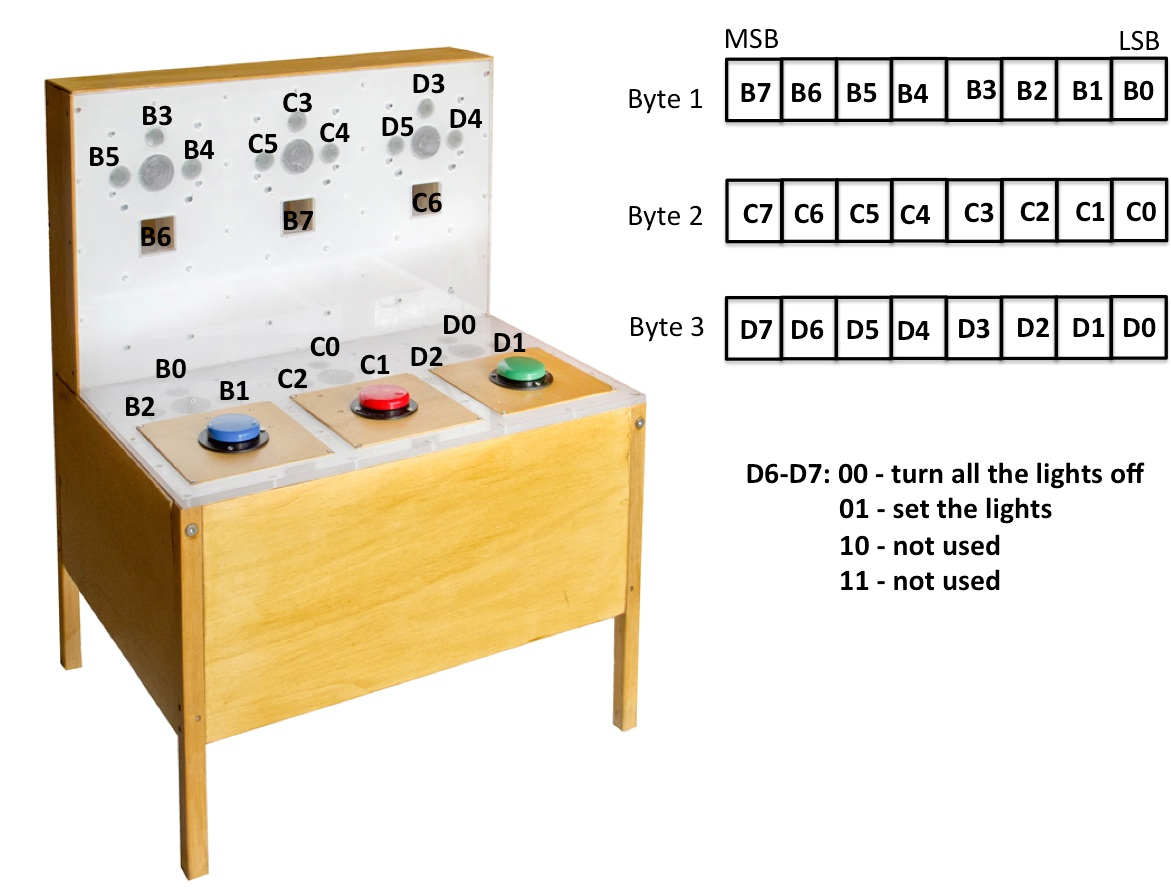
\includegraphics[width=0.8\textwidth]{lights.jpg}
\end{center}
\caption{Experimental board}
\label{fig:experimental_board}
\end{figure}


\begin{itemize}
\item Actions modules which the agent interacts with
\begin{itemize}
\item These are buttons () that can be pressed down
\end{itemize}
\item Rewards modules that are activated according to pre-programmed sequences of the actions modules
\begin{itemize}
\item Lights that switch on/off
\item Small cabinets with lights that can open up
\item Audio feedback
\end{itemize}
\end{itemize}

More details about the board can be found in the IMCLeVeR project website\footnote{http://www.im-clever.eu/}.

The current software interface of the board is written in Labview, and allows the activation of any of the rewards for pre-programmed sequences of actions. Although this control interface provides a quick way of pre-programming the behaviour of the board in a user-friendly way, it has the main limitation that it does not allow dynamic online re-configuration of the board from the controller program of the agent. In our case there was an additional motivation for requiring dynamic control of the board from the controller of the agent; as the available robot platform consisted of only an iCub head, the lack of any actuators prohibited any interaction with the actions modules. For this reason, it was decided to devise a scheme of ``telekinesis'', in which the actions modules could be pushed when the iCub focussed its gaze on them and certain rewards would be given, e.g. lights switch on. As such, we implemented an interface that provides dynamic and online control of the lights rewards through the serial port, and can be used by any controller.

\subsection{Technical}
On the board there is a usb hub which connects a number of I/O usb cards controlling the lights, the buttons, the motors of the rewards draws, the audio, etc. For the serial control interface the I/O cards are connected directly to the usb ports of a PC. The usb-to-serial converter may require a driver which can be found in the manufacturer's website\footnote{http://www.ftdichip.com/Drivers/VCP.htm}, although no installation was necessary as the driver seems to be included in the linux kernel 2.6.32-31, and as such I assume in any more recent ones.

The serial control interface was written in python (2.6.5), and the development platform was running Ubuntu Linux 10.04 64-bit with kernel 2.6.32-31-generic.

The board we had available had a slightly different wiring from the original one shown in Figure~\ref{fig:experimental_board2}. Its differences are highlighted in Figure~\ref{fig:experimental_board2}.
\begin{figure}[htb]
\begin{center}
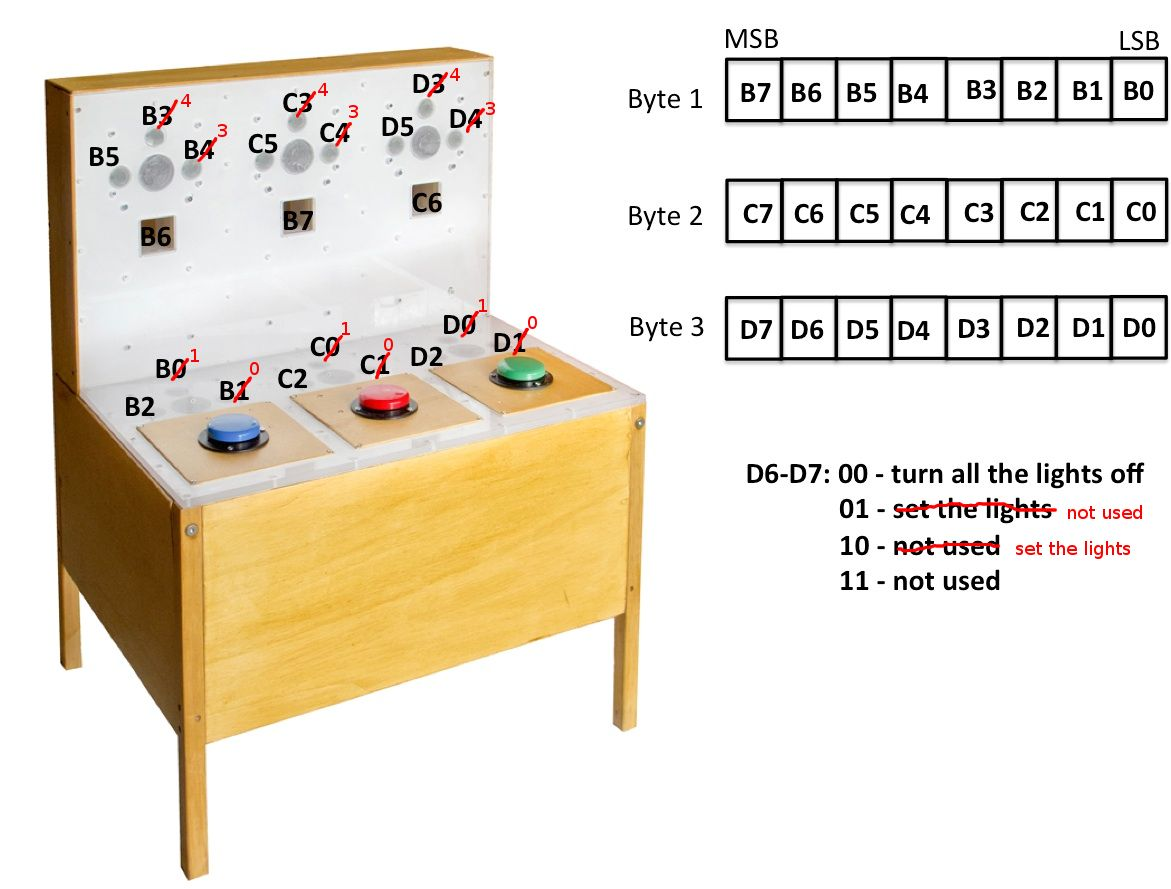
\includegraphics[width=0.8\textwidth]{lights2.jpg}
\end{center}
\caption{Experimental board that was available}
\label{fig:experimental_board2}
\end{figure}

For the control of the lights, the writing of a $3-byte$ message to the (usb-to-)serial port which is connected to the PC is needed. The order of the bits are shown in Figure~\ref{fig:experimental_board2}. The main file is \texttt{board\_serial\_control.py}, which provides the class \texttt{C\_BoardSerialControl} that consists of \texttt{C\_LightsSerialControl} that is responsible for controlling the lights. If the wiring of another board is different from the one provided, all is needed is to change the \texttt{mapping} dictionary (line~60) to the correct mapping. A small utility (\texttt{board\_quick\_test\_serial\_lights.py}) can be used to identify the wiring of your board. Also the programs \texttt{demo.py} and \texttt{demo\_sections.py} demonstrate the use of the provided interface. Lastly, the interface can be easily extended for the rest of the modules on the board if they follow a similar interface.
